\chapter{Stand van zaken}
\label{ch:stand-van-zaken}

\section{Inleiding}

Objectdetectie in domeinspecifieke contexten zoals sonarbeeldvorming wordt vaak gehinderd door een gebrek aan gelabelde data. Traditioneel vereisen gesuperviseerde modellen grote hoeveelheden handmatig gelabelde gegevens om effectieve detectie en classificatie te leren. Semi-supervised en self-supervised learning bieden echter veelbelovende alternatieven door gebruik te maken van grote hoeveelheden ongesuperviseerde data om representaties te leren. Deze literatuurstudie bespreekt de huidige technieken en hun toepassing, met een specifieke focus op de unieke uitdagingen van sonardata.

% Objectdetectie in sonarafbeeldingen
\section{Objectdetectie in sonarafbeeldingen}

\subsection{Definitie en gebruik op sonarafbeeldingen}

Objectdetectie is een tak binnen het domein van computer vision dat gericht is op het identificeren en lokaliseren van objecten binnen beelddata (zoals foto's en video's). Dit wordt gebruikt in verschillende domeinen, zoals beveiligingssystemen (bv. om inbrekers te detecteren) of de medische wereld (bv. om tumoren op te sporen). Door de jaren heen is objectdetectie aanzienlijk geëvolueerd dankzij de vooruitgang in deep learning en de grote beschikbaarheid van datasets met beeldmateriaal. \autocite{He_2016} \\

Objectdetectie combineert twee belangrijke zaken in computer vision: objectlokalisatie en objectclassificatie. Objectlokalisatie bepaalt de positie van objecten, meestal in de vorm van \glspl{bounding_box} \autocite{Tompson_2015}, terwijl objectclassificatie bepaalt tot welke categorie een gedetecteerd object behoort. Samen geeft dit de mogelijkheid tot het herkennen van verschillende soorten objecten op één foto. \\

Objectdetectie heeft vele toepassingen, ook in domeinen die misschien niet zo voor de hand liggend zijn. Één van deze specialisaties binnen de -- algemene -- objectdetectie is objectdetectie op sonardata. Dit domein is over de laatste jaren erg gegroeid, vooral onder invloed van buitenlandse dreigingen. Zo wordt sonarobjectdetectie gebruikt voor het opsporen van mijnen in zee om ze later onschadelijk te kunnen maken. Naast detectie van mijnen wordt   de techniek ook gebruikt voor verschillende soorten onderzoeken, zoals archeologisch en maritiem onderzoek. Bij deze verschillende toepassingen wordt natuurlijk telkens een kleine variatie op deze techniek gebruikt om telkens andere dingen op te sporen. \autocite{Wang_2024} \\

Traditioneel worden supervised-learning methoden gebruikt voor objectdetectie. Voorbeelden van populaire architecturen binnen dit domein zijn onder andere Faster \gls{rcnn}, \gls{yolo} en \gls{ssd}. \autocite{Redmon_2016} Omdat dit supervised-learning modellen zijn, presteren  ze uitstekend bij voldoende gelabelde data. De annotatiekosten en tijdsinvestering vormen echter een grote belemmering, vooral bij complexe datasets zoals sonar. Sonardata vereist namelijk gespecialiseerde kennis voor het labelen, wat de annotatie nog uitdagender maakt. \autocite{Long_2015} \\

\subsection{Typische uitdagingen bij sonarobjectdetectie}

\lipsum[1-3]

\subsection{Overzicht van bestaande technieken}

Grofweg zijn er twee soorten stromingen die toegepast worden om objectdetectie op sonarafbeeldingen te doen. Enerzijds zijn er de klassieke methoden en anderzijds zijn er de moderne deep learning-technieken. De klassieke methoden werden vooral gebruikt in een tijd waar grote, complexe neurale netwerken trainen onmogelijk was bij gebrek aan voldoende computerkracht, maar worden de dag van vandaag nog altijd gebruikt als pre-processing technieken voor de datasets waarmee de moderne neurale netwerken getraind worden. Deze klassieke methoden berusten enkel op statistische technieken om zo objecten in afbeeldingen te proberen detecteren. Specifiek zijn deze vooral gericht op het verbeteren van beeldkwaliteit en het onderscheiden van objecten van de achtergrond.

\subsubsection{Filtertechnieken}

Een voorbeeld van een klassieke methode zijn filtertechnieken. Deze worden toegepast om ruis in sonarafbeeldingen te verminderen en de beeldkwaliteit te verbeteren. Er bestaan immens veel verschillende soorten filters die elk geoptimaliseerd voor een specifiek doel. Een veelgebruikte filtermethode is het gebruik van adaptieve filters die zich aanpassen aan de lokale kenmerken van het beeld. Een voorbeeld hiervan is te vinden in een artikel van \textcite{Aridgides_1995}. Merk op dat dit inderdaad een relatief oude publicatie is, wat aantoont dat deze technieken al gebruikt werden toen deep learning-gebaseerde objectdetectie niet mogelijk was. \\

In dit artikel introduceren de auteurs een adaptieve filtertechniek die ontwikkeld is om mijnachtige doelen te onderscheiden van achtergrondruis in sonarbeelden. De filter onderdrukt achtergrondruis terwijl het de target behoudt. De procedure omvat vier stappen: het berekenen van een genormaliseerde gemiddelde target, het bepalen van de covariantiematrix van de achtergrondruis, het oplossen van normale vergelijkingen om een adaptief filter te verkrijgen en het toepassen van een 2D-filter op de gegevens. Dit algoritme bewijst dat, hoewel er geen gebruik gemaakt wordt van deep-learningtechnieken, ze toch complex kan zijn. De techniek heeft in verschillende testen prestaties geleverd die vergelijkbaar zijn met die van een ervaren sonaroperator. \\

Adaptieve filters worden ook vandaag de dag nog gebruikt, wat aangetoond wordt door een paper van \textcite{Lourey_2017}. Hierin wordt ook een filtertechniek beschreven die toegepast kan worden op \gls{cas} om interferentie van de directe transmissie en de echo van de target van elkaar te onderscheiden. Deze methode kan als effectieve pre-processing techniek gebruikt worden voor trainingsdata.

\subsubsection{Thresholding}

Naast filtering bestaan er nog andere klassieke methoden. Een \emph{straightforward}-aanpak is een simpele \emph{threshold}. Thresholding is een techniek waarbij pixelwaarden worden vergeleken met een bepaalde drempelwaarde om objecten van de achtergrond te scheiden. Een klassieke benadering is de Otsu-methode, die de interklassevariantie minimaliseert om een optimale drempelwaarde te bepalen. Deze methode wordt beschreven in een artikel van \textcite{Otsu_1979}.

\begin{figure}[H]
    \centering
    \begin{subfigure}{.5\textwidth}
        \centering
        \captionsetup{justification=centering}
        \includegraphics[width=0.9\linewidth]{img_pre_otsu.jpg}
        \caption[Afbeelding voor Otsu's thresholding]{Afbeelding voor Otsu's thresholding}
        \label{fig:img_pre_otsu}
    \end{subfigure}%
    \begin{subfigure}{.5\textwidth}
        \centering
        \captionsetup{justification=centering}
        \includegraphics[width=0.9\linewidth]{img_post_otsu.jpg}
        \caption[Afbeelding na Otsu's thresholding]{Afbeelding na Otsu's thresholding}
        \label{fig:img_post_otsu}
    \end{subfigure}
    \caption[Afbeelding voor en na Otsu's thresholding]{Afbeelding voor en na Otsu's thresholding}
    \label{fig:imgs_otsu}
\end{figure}

Hoewel deze techniek oorspronkelijk is ontwikkeld voor visuele beelden, is deze ook toegepast op sonarafbeeldingen, zoals besproken in verschillende artikels, waaronder dat van \textcite{Yuan_2016} en dat van \textcite{Dimitrova_Grekow_2017}. Ondanks zijn simpliciteit kan deze techniek aanzienlijke verbeteringen teweegbrengen. Dit wordt onder andere aangehaald in een paper van \textcite{Komari_Alaie_2018}. Deze paper onderzoekt objectdetectie met passieve sonar in de Perzische Golf. Aangezien deze binnenzee ondiep is, is er sprake van een hoge hoeveelheid fouten tijdens de detectie. Een bepaald soort adaptieve thresholding-techniek kon de \gls{precision} van hun objectdetectiemodel met 24\% verbeteren.

\subsubsection{Edge detection}

Edge detection is een andere klassieke techniek die wordt gebruikt om de contouren van objecten in sonarafbeeldingen te identificeren. \autocite{Torre_1986} Een bekende methode is de Canny edge detector, die randen detecteert door het maximaliseren van de gradiëntgrootte. Deze techniek komt als beste uit de vergelijkende studie van \textcite{Awalludin_2022}. \\

De Canny edge detector werkt in meerdere stappen om nauwkeurige en robuuste contourdetectie te realiseren. De eerste stap is Gaussian blurring, waarbij het beeld wordt vervaagd om ruis te verminderen en kleine details die geen significante randen vormen te onderdrukken. Vervolgens wordt de gradiënt van het beeld berekend met behulp van Sobel-operatoren in zowel de horizontale als verticale richting, waardoor de randen worden geaccentueerd. Daarna wordt non-maximum suppression toegepast, waarbij alleen de sterkste randen worden behouden en omliggende pixels met lagere gradiëntwaarden worden onderdrukt. De laatste stap is hysteresis thresholding, waarbij twee drempelwaarden worden gebruikt: pixels met een gradiëntsterkte boven de hoge drempel worden als randen geclassificeerd, terwijl pixels onder de lage drempel worden genegeerd. Pixels met tussenliggende waarden worden alleen als rand beschouwd als ze verbonden zijn met een sterke randpixel. Dankzij deze gefaseerde aanpak is de Canny-methode effectief in het detecteren van duidelijke randen, zelfs in ruisgevoelige omgevingen zoals sonarafbeeldingen. \autocite{Ding_2001} \\

Ook edge detection wordt vandaag de dag nog gebruikt om een grote bijdrage te leveren aan bijvoorbeeld segmentatiemodellen. Het onderzoek van \textcite{Priyadharsini_2019} gebruikt gespecialiseerde edge detection als pre-processing voor de data naar een objectdetectiemodel gaat. \\

Deze klassieke technieken vormen de basis voor objectdetectie in sonarafbeeldingen en hebben bijgedragen aan de ontwikkeling van meer geavanceerde methoden. Ze blijven relevant, vooral in situaties waarin resources beperkt zijn of wanneer eenvoud en interpretatie van het model belangrijk zijn. Ze worden tot op de dag van vandaag gebruikt als pre-processing stap, bijvoorbeeld. Doordat computerkracht steeds goedkoper en meer beschikbaar werd, wordt tegenwoordig vaak gekozen voor deep learning-oplossingen voor deze problemen. Er zijn gespecialiseerde architecturen ontwikkeld om objectdetectie uit te voeren. Hieronder worden er enkele besproken.

\subsubsection{YOLO}

\GLS{yolo} is een deep learning-gebaseerde architectuur voor objectdetectie dat bekend staat om zijn snelheid en efficiëntie. Het werd voor het eerst geïntroduceerd in een artikel van \textcite{Redmon_2016} en is sindsdien één van de populairste algoritmes in computervisie. In tegenstelling tot traditionele detectiemethoden, waar objecten in meerdere stappen geanalyseerd worden, verwerkt YOLO een afbeelding in één enkele \emph{pass} van het neurale netwerk. Dit zorgt ervoor dat real-time objectdetectie mogelijk is, waardoor het bijzonder geschikt is voor toepassingen zoals autonome voertuigen, videobewaking en \gls{ar}.

\begin{figure}[H]
    \centering
    \includegraphics[width=\textwidth]{yolo_architecture.png}
    \caption[Originele YOLO-architectuur.]{\label{fig:yolo_architecture}Schematische voorstelling van de originele YOLO-architectuur. \autocite{Redmon_2016}}
\end{figure}

\gls{yolo} gebruikt een \gls{cnn} om objecten direct te lokaliseren en classificeren, wat bijdraagt aan de hoge nauwkeurigheid en snelheid van het model. De eerste stap is het herschalen van de afbeelding naar 448 $\times$ 448 pixels. Daarna wordt één \gls{cnn} op de afbeelding toegepast en ten slotte wordt \gls{nms} toegepast. Met de nieuwste versies, zoals YOLOv4 en YOLOv5, zijn verdere verbeteringen in precisie en rekenkundige efficiëntie doorgevoerd, waardoor het een krachtig hulpmiddel blijft in de wereld van kunstmatige intelligentie.

\subsubsection{Faster R-CNN}

\lipsum[1]

\subsubsection{SSD}

\lipsum[1]

\subsection{Specifieke toepassingen}

\lipsum[1-3]

% Semi-supervised learning: principes en technieken
\section{Semi-supervised learning: principes en technieken}

\subsection{Definitie en waarde binnen objectdetectie}

Binnen het domein van machine learning bestaan er verschillende technieken om een model te trainen. Meestal wordt er gesproken van twee grote stromingen: supervised learning en unsupervised learning. Bij supervised learning wordt er gebruik gemaakt van een dataset en een uitkomst (hetgeen het model uiteindelijk moet kunnen voorspellen). Dit kan een label zijn of een bepaalde numerieke waarde. Belangrijk is dat zowel de input als de gewenste output gegeven zijn. Het model leert dus het verband tussen de twee. Bij unsupervised learning zijn er geen verwachte outputs. De volledige dataset wordt door het model gebruikt om patronen in te herkennen. Unsupervised learning wordt daarom ook meestal gebruikt om verkennende data-analyse uit te voeren. Echter hebben beide methoden enkele nadelen. Bij supervised learning is het traag en duur om alle data op een correcte manier te labelen. Unsupervised learning heeft dit probleem niet, maar heeft een beperkt aantal toepassingen en is minder accuraat. Een alternatief is \gls{ssl}, wat een compromis tussen zowel supervised als unsupervised learning is. \autocite{C_A_Padmanabha_Reddy_2018} \\

\gls{ssl} is een subdomein van machine learning waar gebruik gemaakt wordt van zowel gelabelde als ongelabelde data om modellen te trainen. Dit is bijzonder nuttig in situaties waarin het labelen van gegevens duur of tijdrovend is, zoals bij sonardata het geval is. \gls{ssl} bevindt zich tussen supervised learning (waar alle trainingsdata gelabeld zijn) en unsupervised learning (waar geen labels beschikbaar zijn). Door gebruik te maken van een kleine hoeveelheid gelabelde gegevens in combinatie met een grote hoeveelheid ongelabelde gegevens, kan een model beter generaliseren waardoor de prestaties verbeteren met minder menselijke annotatie-inspanning. \autocite{Hady_2013} \\

Zoals eerder vermeld, is \gls{ssl} een subdomein van machine learning, net zoals supervised en unsupervised learning. Het is dus niet één model of één architectuur, maar een waaier van verschillende algoritmen die soms op hele andere manieren werken. Wel hebben ze allemaal gemeen dat ze zowel gelabelde als ongelabelde data gebruiken. \\

Één van de belangrijkste technieken binnen \gls{ssl} is \emph{consistency regularization} (cf. infra), waarbij een model wordt aangemoedigd om consistente voorspellingen te maken voor kleine verstoringen van dezelfde ongelabelde input. \autocite{Fan_2022} Een ander veelgebruikt principe is \emph{pseudo-labeling} (cf. infra), waarbij het model zelf voorspellingen genereert voor ongelabelde gegevens en deze gebruikt als extra trainingsdata. \autocite{Lee_2013} \\

Daarnaast is er graph-based \gls{ssl}. Dit is een techniek die gebruik maakt van grafen (netwerken) om de relaties tussen gelabelde en ongelabelde data te modelleren en labelinformatie effectiever te verspreiden. In plaats van uitsluitend te vertrouwen op individuele gegevenspunten, gebruiken deze methoden de structuur van de dataset om aannames te maken over onbekende labels. Dit is vooral nuttig in situaties waarin de onderliggende data een natuurlijke connectiviteit vertoont, zoals sociale netwerken, biologische netwerken en tekstanalyses. \autocite{Song_2021} \\

Graph-based \gls{ssl}-modellen stellen de dataset voor als een graaf $G = (V, E)$ waarbij $V$ de knopen (datapunten) zijn (zowel gelabelde als ongelabelde gegevens) en $E$ de de gewogen randen (connecties) tussen knopen zijn, die de relatie of gelijkenis tussen de datapunten aangeven. Het basisidee is dat naburige knopen waarschijnlijk tot dezelfde klasse behoren, een principe dat bekend staat als \emph{label propagation}. Labels van bekende knopen (gelabelde data) worden hierbij iteratief verspreid naar naburige knopen op basis van de sterkte van de verbindingen. \autocite{Zhu_2005} \\

\gls{ssl} wordt toegepast in diverse domeinen, zoals beeld- en spraakherkenning, biomedische analyse en autonome systemen. Recente ontwikkelingen in deep learning hebben geleid tot geavanceerde \gls{ssl}-methoden, zoals FixMatch en MixMatch (cf. infra), die de prestaties aanzienlijk verbeteren door sterke data-augmentatie, efficiënter gebruik van ongelabelde data en de combinatie van andere \gls{ssl}-technieken. Onderzoek heeft aangetoond dat \gls{ssl} met slechts 10\% gelabelde data al bijna dezelfde prestaties kan bereiken als volledig gelabelde modellen. \autocite{Lucas_2022}

\subsection{Veelgebruikte SSL-methoden}

\acrfull{ssl} omvat verschillende methoden die gebruik maken van zowel gelabelde als ongelabelde data om de prestaties van machine learning-modellen te verbeteren. Veelgebruikte \gls{ssl}-methoden compenseren de beperkte beschikbaarheid van gelabelde data door patronen en structuren in ongelabelde data te benutten. \gls{ssl} wordt voor alle soorten doeleinden gebruikt: niet alleen in predictieve modellen, waarbij er vaak gebruik gemaakt wordt van pseudo-labeling en consistency regularization, wordt \gls{ssl} ingezet. Ook bij generatieve modellen wordt \gls{ssl} enorm veel gebruikt. Dit gaat dan bijvoorbeeld om \glspl{vae} en \glspl{gan}. Deze worden hierbij ingezet om aanvullende trainingsgegevens te genereren. Door al deze technieken te combineren, kunnen \gls{ssl}-methoden significante verbeteringen bieden voor taken zoals beeldherkenning, spraakverwerking en \gls{nlp}. \autocite{van_Engelen_2019} Hieronder worden enkele van de meest prominente technieken binnen \gls{ssl} besproken.

\subsubsection{Pseudo-labeling}

Pseudo-labeling is een belangrijke techniek binnen \gls{ssl} waarbij een model, getraind op een beperkte hoeveelheid gelabelde data, wordt ingezet om voorspellingen te doen op ongelabelde data. Deze voorspellingen, aangeduid als ``pseudo-labels'', worden vervolgens behandeld als echte labels, waardoor het model verder kan worden verfijnd met een uitgebreidere dataset. Dit proces wordt iteratief herhaald, zodat het model geleidelijk aan zijn prestaties verbetert door zowel de gelabelde als de pseudo-gelabelde data te gebruiken. \autocite{Lee_2013} \\

Het succes van pseudo-labeling is natuurlijk afhankelijk van de nauwkeurigheid van de gegenereerde pseudo-labels. Om de kwaliteit te waarborgen, wordt vaak een drempelwaarde ingesteld voor de voorspellingszekerheid: alleen voorspellingen die boven deze drempel uitkomen, worden als pseudo-labels geaccepteerd. Dit helpt het model om zich te concentreren op voorbeelden waarbij het relatief zeker is van de voorspelling, waardoor het risico op het leren van verkeerde informatie wordt verminderd. \autocite{Kage_2024} \\

Een belangrijk voordeel van pseudo-labeling is dat het effectief gebruikmaakt van grote hoeveelheden ongelabelde data, wat vooral nuttig is in domeinen zoals sonarbeeldvorming, waar het verkrijgen van gelabelde data duur en tijdrovend is. Verder zijn toepassingen van pseudo-labeling te vinden in verschillende gebieden, waaronder beeldherkenning, spraakverwerking en \gls{nlp}. \autocite{Min_2022} Recent onderzoek van \textcite{Ferreira_2023} heeft aangetoond dat pseudo-labeling een zeer goede performantie kan neerzetten, terwijl het de behoefte aan uitgebreide gelabelde datasets vermindert. \\

Desondanks kent pseudo-labeling ook uitdagingen. Als het model in een vroeg stadium onnauwkeurige pseudo-labels genereert, kan dit leiden tot het versterken van fouten, een fenomeen bekend als \emph{confirmation bias}. Om dit te voorkomen, worden technieken zoals \emph{curriculum learning} toegepast, waarbij het model eerst wordt getraind met de meest zekere pseudo-labels en geleidelijk aan minder zekere voorbeelden toevoegt naarmate de training vordert. \autocite{Cascante_Bonilla_2020}

\subsubsection{Consistency Regularization}

Een ander fundamenteel concept binnen \gls{ssl} is consistency regularization. Deze techniek wordt in verschillende algoritmen gebruikt om de betrouwbaarheid van het model te verbeteren. Het doet dit door het model te dwingen consistente voorspellingen te maken voor kleine variaties van dezelfde input. Het idee is gebaseerd op de veronderstelling dat een model robuust moet zijn tegen kleine verstoringen in de input, vooral wanneer de input geen gelabelde gegevens bevat. \\

Eerst wordt een ongelabeld voorbeeld $x_u$ aangepast met kleine verstoringen. Dit kan gaan om data-augmentatie (bv. willekeurige rotaties, verscherping, kleuraanpassingen, \dots), het toevoegen van ruis (bv. Gaussian noise), \dots Dit resulteert in twee versies van dezelfde input: het origineel $x_u$ en de verstoorde versie $x'_u$. Daarna voorspelt het model de kansverdeling van de klassen voor zowel de originele als de verstoorde input. \\

Een consistente voorspelling betekent dat beide kansverdelingen ``dicht'' bij elkaar moeten liggen. Om dit te garanderen wordt een gespecialiseerde \gls{loss_functie} gebruikt, zoals de \gls{kl}-divergentie \autocite{Hall_1987} of de \gls{mse}. Het model wordt getraind om deze \emph{loss} te minimaliseren, zodat het stabiele en robuuste voorspellingen leert maken, zelfs bij verstoringen. \\

Consistency regularization is enorm effectief (en wordt daarom ook veel gebruikt) omdat het ervoor zorgt dat het model gebruik maakt van de onderliggende structuur van ongelabelde data. Hierdoor verbetert de generalisatie, omdat het model minder gevoelig wordt voor kleine ruis en variaties. Daarnaast verhoogt de sample-efficiëntie, waardoor minder gelabelde data nodig is voor goede prestaties. \autocite{Fan_2022}

\subsubsection{FixMatch}

Beide voorgaande technieken -- zowel pseudo-labeling als consistency regularization -- zijn slechts concepten binnen het domein van \gls{ssl}. Dit wil daarom niet zeggen dat ze niet gebruikt worden in productie, maar vaak zijn ze slechts steunpilaren voor een grotere, complexere en effectievere architecturen. Hieronder wordt FixMatch -- een eerste voorbeeld die relevant is voor dit onderoek -- besproken. \\

FixMatch combineert pseudo-labeling met consistency regularization. Het werd geïntroduceerd door \textcite{Sohn_2020} en heeft bewezen indrukwekkende prestaties te leveren op benchmarks zoals CIFAR-10, waarbij met slechts 250 gelabelde voorbeelden een nauwkeurigheid van 94,93\% werd bereikt. De kernideeën achter FixMatch zijn gebaseerd op het principe dat een model consistente voorspellingen zou moeten maken, zelfs wanneer invoerdata wordt gewijzigd met verschillende vormen van data-augmentatie. FixMatch combineert twee belangrijke technieken binnen \gls{ssl}: pseudo-labeling en sterke versus zwakke augmentatie. \\

Voor een gegeven ongelabeld voorbeeld $x_u$ wordt eerst een zwak geaugmenteerde versie $x_u^w$ gegenereerd met eenvoudige transformaties zoals willekeurige spiegelingen en verschuivingen. Het model maakt een voorspelling $p\left(y|x_u^w\right)$, wat een kansverdeling over de mogelijke klassen oplevert. Als de hoogste voorspelde waarschijnlijkheid boven een drempel $\tau$ ligt wordt dit label als pseudo-label gebruikt. 

$$
\hat{y}_u = \arg \max p\left(y|x_u^w\right) \ \text{indien} \ \max p\left(y|x_u^w\right) > \tau
$$

Dit voorkomt dat onzekere voorspellingen als pseudo-labels worden gebruikt, waardoor ruis in de trainingsdata wordt verminderd. \\

Vervolgens wordt een sterk geaugmenteerde versie $x_u^s$ van dezelfde input $x_u$ gemaakt met agressieve augmentaties, zoals kleurvervormingen en Cutout (willekeurige afdekking van delen van de afbeelding). \autocite{DeVries_2017} Het model wordt getraind om dezelfde voorspelling $\hat{y}_u$ te maken op de sterk geaugmenteerde input $x_u^s$, waardoor het robuust wordt tegen verschillende variaties in de data. \\

Om FixMatch te trainen is er echter een gespecialiseerde \gls{loss_functie} nodig, die een combinatie is voor zowel de gelabelde als de pseudo-gelabelde data:

$$
L = L_s + \lambda_u L_u
$$

waarbij $L_s$ de gewone \gls{loss_functie} is voor de gelabelde data, $L_u$ de \emph{consistency loss} is voor pseudo-gelabelde data, gedefinieerd als de gemiddelde cross-entropy tussen het pseudo-label en de voorspelling op $x_{u'}^s$ en $\lambda_u$ een hyperparameter is die de balans tussen gelabelde en ongelabelde data regelt. \\

De hoge performantie van FixMatch heeft verschillende redenen: In tegenstelling tot traditionele pseudo-labeling, waarbij alle voorspellingen worden gebruikt, accepteert FixMatch alleen pseudo-labels als de modelvoorspelling een zekerheid boven een vooraf ingestelde drempel $\tau$ heeft. Dit voorkomt het versterken van foute pseudo-labels en verbetert de robuustheid van het model. Ook wordt het model gedwongen om dezelfde voorspelling te maken voor een input, ongeacht of deze zwak of sterk geaugmenteerd is. Dit helpt het model om stabiele, generaliseerbare representaties te leren. Daarnaast voorkomt het toepassen van een tweefasige-augmentatiestrategie dat het model te afhankelijk wordt van specifieke kenmerken in de data. Dit helpt overfitting te verminderen.

\subsubsection{MixMatch}

MixMatch integreert ook verschillende \gls{ssl}-technieken, waaronder data-augmentatie, pseudo-labeling en mixup. Het algoritme is een verbetering op de FixMatch-architectuur en werd geïntroduceerd door \textcite{Berthelot_2019}. In benchmarks heeft het hele goede prestaties geleverd op datasets zoals CIFAR-10 en STL-10. \\

Voor elk ongelabeld voorbeeld wordt het model meerdere keren toegepast om voorspellingen te genereren. Het gemiddelde van de voorspellingen wordt gebruikt om ruis te verminderen en betrouwbaardere pseudo-labels te verkrijgen. Dit helpt het model om robuustere pseudo-labels te creëren dan traditionele pseudo-labeling, waar slechts één voorspelling per voorbeeld wordt gebruikt. \\

Om ervoor te zorgen dat de pseudo-labels niet te onzeker zijn, wordt een \emph{softmax-temperature-scaling} toegepast om de kansverdeling scherper te maken. Dit betekent dat het model meer vertrouwen krijgt in de meest waarschijnlijke klassen, waardoor het pseudo-label effectiever wordt.

$$
q(y|x) = \frac{p(y|x)^{\frac{1}{T}}}{\sum_{y'} p(y'|x)^\frac{1}{T}}
$$

waarbij $T$ de temperatuurparameter is die de scherpte van de distributie regelt (kleinere waarden leiden tot scherpere distributies). \\

MixMatch maakt ook gebruik van \emph{mixup}, een data-augmentatietechniek waarbij synthetische trainingssamples worden gemaakt van paren bestaande trainingssamples en hun labels ($(x_1, y_1)$ en $(x_2, y_2)$). Merk op dat zowel de gelabelde als de pseudo-gelabelde samples gebruikt worden. 

\begin{align*}
    \tilde{x} & = \lambda x_1 + (1 - \lambda) x_2 \\
    \tilde{y} & = \lambda y_1 + (1 - \lambda) y_2
\end{align*}

Hierbij is $\lambda$ een gewichtsparameter, die willekeurig gekozen is uit een Beta-verdeling. Deze techniek zorgt voor soepelere beslissingsgrenzen en vermindert overfitting door het model te dwingen om robuuster te generaliseren. \autocite{Zhang_2017} \\

Omdat dezelfde input meerdere keren wordt geaugmenteerd en verwerkt, wordt het model getraind om consistente voorspellingen te maken voor deze variaties. Dit dwingt het model om stabiele representaties te leren, zelfs wanneer kleine veranderingen worden aangebracht in de inputdata. Net zoals FixMatch minimaliseert MixMatch een gecombineerde \gls{loss_functie} die zowel de gelabelde als de pseudo-gelabelde voorbeelden gebruikt (cf. supra). \autocite{Berthelot_2019}

% Self-supervised learning: principes en technieken
\section{Self-supervised learning: principes en technieken}

\subsection{Definitie en verschil met SSL}

\lipsum[1]

\subsection{Werking}

\lipsum[1]

\subsection{Veelgebruikte Self-SL methoden}

\lipsum[1]

\subsubsection{SimCLR}

\lipsum[1]

\subsection{MoCo}

\lipsum[1]

\subsection{BYOL}

\lipsum[1]

% Vergelijking van relevante methoden
\section{Vergelijking van relevante methoden}

%TODO: Schrijven 'Vergelijking van relevante methoden'
\lipsum[1-3]

% Faster R-CNN
\autocite{Wang_2023}
\autocite{Zeng_2021}
\autocite{Yulin_2020}
\autocite{Chen_2017}

% Overzicht van bestaande datasets en annotatietechnieken
\section{Overzicht van bestaande datasets en annotatietechnieken}

\subsection{Beschikbaarheid van publieke datasets}

Zoals al eerder vermeld, is er voor het trainen van een objectdetectiemodel een substantiële hoeveelheid gelabelde data nodig. Tegenwoordig worden veel datasets -- zo goed als volledig geprepareerd voor het trainen van ML-modellen -- online aangeboden onder een vrije licentie. Dit zorgt ervoor dat de datasets opnieuw gepubliceerd en hergebruikt mogen worden met weinig tot geen beperkingen. Het concept van \emph{Open Data} wordt de laatste jaren steeds populairder, aangezien onderzoek zich hoe langer hoe meer ook naar het internet verplaatst. \autocite{Murray_Rust_2008} \\

Platformen zoals \href{https://www.kaggle.com/datasets}{Kaggle} of \href{https://huggingface.co/datasets}{Hugging Face} hebben zich gespecialiseerd in het verspreiden van deze open datasets en kunnen rekenen op een hele community van gebruikers om deze datasets te uploaden naar hun platformen. Ook verschillende overheidsorganisaties en onderzoeksinstellingen maken veel van hun data openbaar. Voorbeelden hiervan zijn \href{https://data.europa.eu/}{data.europa.eu} voor het dataplatform van de Europese Unie, \href{https://data.gov.be/nl}{data.gov.be} voor het Belgische Data Portaal en \href{https://data.gov/}{data.gov} voor open data van de Amerikaanse overheid. \\

Voor datasets over niche onderwerpen zijn de mogelijkheden vaak beperkter. Dit heeft verschillende redenen: eerst en vooral zijn er minder mensen met deze onderwerpen bezig, wat de kan automatisch kleiner maakt dat ze (grote) datasets gaan verzamelen en deze publiek beschikbaar maken. Ten tweede brengt een dataset samenstellen een aanzienlijke kost met zich mee, zeker wanneer deze \textit{from scratch} gemaakt moet worden en men zich bijvoorbeeld niet kan baseren op reeds bestaande datasets. Ten derde is het vaak zo dat deze zeer gespecialiseerde datasets confidentieel moeten blijven, aangezien het bijvoorbeeld gaat over gevoelige data of data over een technologie die nog volop in ontwikkeling is.

\subsection{Problemen bij sonardatasets}

Sonardata leidt aan alle drie deze problemen. Sonardata van de zeebodem moet namelijk met een gespecialiseerde \GLS{auv} verzameld worden. Anders dan bij een \GLS{rov} kan deze volledig autonoom opereren en is daarom zeer geschikt om sonaropnames te maken. Weinig bedrijven hebben echter een nuttige reden om de kost hiervan te kunnen rechtvaardigen. Daarnaast is er namelijk nog een hele crew en een schip nodig om dergelijk onderzoek uit te voeren. Toch zijn er organisaties die deze nood hebben aan deze data. Specifiek gaat dit dan over onderzoeksinstellingen die bepaalde dingen op de zeebodem onderzoeken. Maar ook Defensie en Marine kunnen zulke data enorm goed gebruiken voor veiligheidsdoeleinden. AUV's worden in deze context gebruikt om bijvoorbeeld zeemijnen op te sporen, in kaart te brengen en onschadelijk te maken. \\

Ook worden ze gebruikt om te patrouilleren: ze kunnen hierbij kritieke infrastructuur zoals haveningangen en zeekabels bewaken en zorgen dat deze veilig en onbeschadigd blijven. Dit brengt natuurlijk onmiddellijk het derde probleem met zich mee. Alle data die door Defensie of Marine is verzameld, is automatisch confidentieel en mag onder geen enkele voorwaarde gebruikt -- laat staan gepubliceerd -- worden voor andere doeleinden. Data van de zeebodem -- en van mijnen of kritieke infrastructuur -- is namelijk van onschatbare waarde voor een potentiële vijand. \autocite{Aubard_2024_Datasets}

\subsection{Mogelijke oplossingen}

Deels omwille van de niche, deels door de hoge kosten van de apparatuur en deels door de hoge graad van gegevensbescherming is er dus nagenoeg geen -- kwalitatieve -- sonardata vrij beschikbaar. Dit is echter ook nadelig voor verdere ontwikkeling binnen het domein. Daarom zijn er -- nog maar heel recent -- enkele initiatieven opgekomen om dit alsmaar groter wordend probleem te proberen oplossen. \\

In een artikel van \textcite{Aubard_2024_Datasets} gepubliceerd in IEEE Journal of Oceaning Engineering wordt het probleem aangehaald en worden enkele oplossingen aangereikt om om te gaan met de schaarste. Daarnaast wordt een vergelijking gemaakt van (bijna) alle sonardatasets -- die overigens nog maar heel recent publiek beschikbaar zijn. Er worden in het artikel verschillende soorten datasets voor verschillende doeleinden gepresenteerd. Zo is er een aanbod van verschillende soorten sonar, verschillende formaten van data, verschillende hoeveelheden data, verschillende types objecten in de data en data voor verschillende doeleinden (zoals classificatie, objectdetectie, segmentatie, \dots). \\

In dit onderzoek wordt de focus gelegd op objectdetectie. Hierdoor vallen er al veel datasets af. Er blijven nog zo'n 5 datasets over die mogelijks gebruikt kunnen worden.

\begin{table}[H]
    \centering
    \begin{tabular}{lllll}
        \toprule
        \textbf{Dataset} & \textbf{Sonar} & \textbf{Hoeveelheid} & \textbf{Object labels} & \textbf{Jaar} \\
        \midrule
        UATD                   & FLS & 9200  & Banden, Kooien, \glspl{rov} & 2022 \\
        SSS for Mine Detection & SSS & 1170  & Mijnen                      & 2024 \\
        SWDD                   & SSS & 7904  & Muren                       & 2024 \\
        SubPipe                & SSS & 10030 & Pijpleidingen               & 2024 \\
        UXO                    & FLS & 74437 & \Glspl{blindganger}         & 2024 \\
        \bottomrule
    \end{tabular}
    \caption[Mogelijke datasets]{\label{tab:possible_datasets} Tabel van mogelijk bruikbare datasets voor dit onderzoek.}
\end{table}

Merk op dat al deze datasets nog niet lang geleden zijn gepubliceerd, wat er op wijst dat er slechts heel recent aandacht wordt besteed aan dit specifieke probleem. Op zich zijn al deze datasets van dermate kwaliteit dat ze kunnen dienen om een objectdetectiemodel te trainen. Echter vallen bepaalde datasets buiten de scope van dit onderzoek, zoals de SWDD dataset. Deze dataset is gemaakt voor de ontwikkeling van het ROSAR-framework in een paper van \textcite{Aubard_2024_ROSAR}. Ze is echter minder geschikt om te gebruiken in dit onderzoek, aangezien het namelijk sonarbeelden die gemaakt zijn door een \gls{auv} alle havenmuren van de haven van Porto de Leixões in Portugal te laten volgen en deze af te scannen bevat. \autocite{Aubard_2024_SWDD} \\

Ook de SubPipe-dataset biedt geen echte meerwaarde voor dit onderzoek. Ze bevat namelijk beelden voor de inspectie van pijpleidingen. Echter bewijst deze dataset wel dat er door de initiatieven van de afgelopen jaren datasets ter beschikking gesteld zijn met voldoende data om een robuust model mee te trainen. SubPipe bevat ongeveer 80GB aan data, verdeeld in data voor SLAM, objectdetectie en segmentatie. Ook worden er (normale) foto's in hoge resolutie (gemaakt met een GoPro Hero 10) en annotatie/metadata in verschillende formaten meegeleverd. \autocite{Alvarez_Tunon_2024} \\

Zo blijven er nog 3 datasets over die mogelijks geschikt zijn om in dit onderzoek te gebruiken. 

\newpage

\subsubsection{UATD}

De Underwater Acoustic Target Detection-dataset bevat meer dan 9000 \gls{mfls}-sonarbeelden. Ze bevat de \emph{raw} sonardata met annotatie. Er komen 10 verschillende categorieën van \emph{target}-objecten in voor, waaronder kooien, banden en cilinders. De data is -- in tegenstelling tot sommige andere datasets -- verzameld door een \gls{auv} in meren en plassen. De data komt met andere woorden uit ``de echte wereld'', wat voordelig is voor de training van modellen die in \emph{real-world}-scenario's gebruikt zullen worden. \autocite{Xie_2022}

\begin{figure}[H]
    \centering
    \includegraphics[width=\textwidth]{UATD_Objects.png}
    \caption[UATD Objecten.]{\label{fig:uatd_objects}Overzicht van objecten in de UATD-dataset. \autocite{Xie_2022}}
\end{figure}

De dataset wordt verspreid in een figshare-repository onder de CC BY 4.0 licentie. Deze licentie laat de gebruiker toe om het materiaal te delen en te bewerken, ook voor commerciële doeleinden. Buiten een naamsvermelding van de maker, een link naar de licentie en een vermelding of het werk al dan niet veranderd is, zijn er geen verdere restricties. De dataset wordt als ZIP-archief aangeboden. Gecomprimeerd is deze ongeveer 4,47 GB groot. Uitgepakt bevat ze drie aparte datasets en OpenSLT, de annotatietool die gebruikt werd, telkens opnieuw apart verpakt als ZIP-archief. De drie datasets zijn als volgt verdeeld: twee testsets -- \texttt{UATD\_Test\_1} en \texttt{UATD\_Test\_2} -- en één trainingsset -- \texttt{UATD\_Training}. Elk archief -- buiten die van de annotatietool natuurlijk -- bevat twee mappen: \texttt{annotations} en \texttt{images}. De map \texttt{annotations} bevat de annotaties en de map \texttt{images} bevat de sonarbeelden. \autocite{Jian_2022} \\

\begin{table}[H]
    \centering
    \begin{tabular}{llll}
        \toprule
        \textbf{Dataset} & \textbf{Aantal bestanden} & \textbf{Gecomprimeerde grootte} & \textbf{Ware grootte} \\
        \midrule
        UATD\_Test\_1  & 800  & 421.9 MB & 3.3 GB \\
        UATD\_Test\_2  & 800  & 424.6 MB & 3.3 GB \\
        UATD\_Training & 7600 & 3.9 GB   & 25.8 GB \\
        \bottomrule
    \end{tabular}
    \caption[Datasets binnen UATD]{\label{tab:uatd_datasets_overview} Tabel van eigenschappen van de datasets binnen de UATD-dataset. \autocite{Jian_2022}}
\end{table}

De bestanden volgen een vast benamingsschema zodat de beelden en de annotaties makkelijk aan elkaar gekoppeld kunnen worden. In elke dataset zijn de bestanden genummerd van \texttt{00001} tot aan het aantal bestanden in de dataset (bv. \texttt{00800} voor elke testset). Het beeld en de overeenkomstige annotatie hebben hetzelfde nummer. Zo zijn de paden voor het tweede beeld bijvoorbeeld:

\begin{itemize}
    \item \textbf{Beeld:} \texttt{UATD/UATD\_Test\_1/images/00003.bmp}
    \item \textbf{Annotatie:} \texttt{UATD/UATD\_Test\_1/annotations/00003.xml}
\end{itemize}

\begin{figure}[H]
    \centering
    \includegraphics[width=0.5\textwidth]{UATD_example_annotated.png}
    \caption[UATD afbeelding met bounding boxes.]{\label{fig:uatd_image}Voorbeeld van een sonarbeeld binnen de UATD-dataset met de objecten aangeduid met \glspl{bounding_box} (afbeelding \texttt{UATD\_Test\_1/00003}). \autocite{Xie_2022}}
\end{figure}

De beelden zijn opgeslagen als 3-kanaals ongecomprimeerde BMP-bestanden met een bitdiepte van 8 bits (één byte). Dit is één van de eenvoudigste bestandsformaten om een foto op te slaan. Het bestand bevat namelijk een lijst van alle pixels, waarbij voor elke pixel het kleur wordt bijgehouden. Het kleur wordt in dit geval dus opgeslagen in 8 bits. Dit betekent dat het kleur van elke pixel bepaald wordt door een waarde tussen 0 en 255. Aangezien er drie kanalen zijn (RGB: Rood, Groen en Blauw), wordt elke pixel dus beschreven door $8 \times 3 = 24$ bits of 3 bytes. Als de afmetingen van de afbeelding gekend zijn, is het makkelijk om de grootte van de afbeelding te berekenen met behulp van volgende formule:

$$
\text{Grootte in Bytes} = \frac{breedte \times hoogte \times \#kanalen \times bitdiepte}{8}
$$ \\

Naast enkele tientallen bytes aan header- en fotodata is dit de werkelijke grootte van een BMP-bestand. Het nadeel is echter dat zo'n bestand heel snel heel groot wordt, aangezien BMP meestal gebruikt wordt zonder compressie. Anderzijds is zo'n verzameling van BMP-bestanden dan weer heel goed te comprimeren in bijvoorbeeld een ZIP-bestand. Zo kon de UATD-dataset van ongeveer 32,8 GB naar ongeveer 4,75 GB gecomprimeerd worden \footnote{Dit gaat over de som van de drie ZIP-bestanden die nog eens gezipt in de UATD-dataset zaten. De drie bestanden zijn dus nog eens gecomprimeerd, wat de grootte van het origineel gedownloade bestand op 4,47 GB bracht.}, wat op een compressiegraad van ongeveer 6.8 neerkomt. \autocite{Bourke_1998}

\begin{figure}[H]
    \centering
    \begin{tikzpicture}
        % Define parameters
        \def\imgSize{5}   % Image size (6x6 cm)
        \def\cellSize{1}  % Size of each cell
        \def\offset{7}    % Offset for second column
        \def\stackShift{0.5} % Shift for stacking channels
        \def\gridStep{\imgSize/5} % Step size for 6x6 grid
        
        % ==========================
        % First Column (Actual Image)
        % ==========================
        % Insert real image
        \node[anchor=south west, inner sep=0] (img) at (0,0) 
        {\includegraphics[width=\imgSize cm, height=\imgSize cm]{UATD_example.png}};
        
        % Draw white grid overlay (10x10)
        \draw[step=\gridStep,white, thick] (0,0) grid (\imgSize, \imgSize);
        
        % Image dimensions
        \draw[<->, thick] (-0.5, 0) -- (-0.5, \imgSize);
        \node[left] at (-0.5, \imgSize/2) {1028};
        
        \draw[<->, thick] (0, -0.5) -- (\imgSize, -0.5);
        \node[below] at (\imgSize/2, -0.5) {1024};
        
        % ==========================
        % Second Column (RGB Breakdown, Correct Stacking)
        % ==========================
        % 1. Blue Channel (furthest back, largest shift)
        \begin{scope}[shift={(\offset+2*\stackShift, 2*\stackShift)}]
            \fill[blue!50] (0,0) rectangle (\imgSize, \imgSize);
            \draw[white, thick, step=\gridStep] (0,0) grid (\imgSize, \imgSize);
        \end{scope}
        
        % 2. Green Channel (middle layer, medium shift)
        \begin{scope}[shift={(\offset+\stackShift, \stackShift)}]
            \fill[green!50] (0,0) rectangle (\imgSize, \imgSize);
            \draw[white, thick, step=\gridStep] (0,0) grid (\imgSize, \imgSize);
        \end{scope}
        
        % 3. Red Channel (front layer, no shift)
        \begin{scope}[shift={(\offset, 0)}]
            \fill[red!50] (0,0) rectangle (\imgSize, \imgSize);
            \draw[white, thick, step=\gridStep] (0,0) grid (\imgSize, \imgSize);
        \end{scope}
        
        % Dimensions for RGB squares
        \draw[<->, thick] (\offset-0.5, 0) -- (\offset-0.5, \imgSize);
        \node[left] at (\offset-0.5, \imgSize/2) {1028};
        
        \draw[<->, thick] (\offset, -0.5) -- (\offset+\imgSize, -0.5);
        \node[below] at (\offset+\imgSize/2, -0.5) {1024};
        
        % Diagonal arrow for number of channels (bottom-right corner)
        \draw[<->, thick] (\offset+0.7*\stackShift+\imgSize, -0.5) 
        -- (\offset+\stackShift+\imgSize+1, 0.5);
        \node[below] at (\offset+\stackShift+\imgSize+0.85, 0) {3};
        
    \end{tikzpicture}
    \caption[Voorbeeld van een bitmap.]{\label{fig:bitmap_example_image}Voorbeeld van de structuur van een bitmap-afbeelding zoals BMP.}
\end{figure}

Per afbeelding is er steeds een overeenkomstig XML-bestand dat de annotatie bevat. De annotatie volgt het Pascal VOC-formaat. Dit annotatieformaat werd origineel ontwikkeld voor de Visual Object Challenge (VOC). Deze challenge is een benchmark voor classificatie en objectdetectie die sinds 2005 jaarlijks georganiseerd wordt. Ondertussen is het formaat uitgegroeid tot een veelgebruikte standaard voor de annotatie van visuele datasets voor bijvoorbeeld objectdetectie. Door het gebruik van XML is het formaat makkelijk leesbaar. Echter maken heel weinig modellen rechtstreeks gebruik van het Pascal VOC-formaat, waardoor de annotatie meestal moet omgezet worden naar een ander formaat. \autocite{Everingham_2009}

\clearpage

\begin{listing}[H]
    \begin{minted}{xml}
        <annotation>
            <sonar>
                <range>24.9909</range>
                <azimuth>120</azimuth>
                <elevation>12</elevation>
                <soundspeed>1498.1</soundspeed>
                <frequency>1200k</frequency>
            </sonar>
            <file>
                <folder>UATD_Test_1</folder>
                <filename>00004</filename>
            </file>
            <size>
                <width>1024</width>
                <height>1257</height>
                <channel>3</channel>
            </size>
            <object>
                <name>rov</name>
                <bndbox>
                    <xmin>574</xmin>
                    <ymin>880</ymin>
                    <xmax>618</xmax>
                    <ymax>909</ymax>
                </bndbox>
            </object>
        </annotation>
    \end{minted}
    \caption[PASCAL VOC-annotatie]{Voorbeeld van een XML-bestand met annotatie voor objectdetectie in het PASCAL VOC-formaat (annotatie van \texttt{UATD\_Test\_1/00004}). \autocite{Xie_2022}}
\end{listing}

\subsubsection{SSS for Mine Detection}

Een andere mogelijke kandidaat is de \emph{\acrshort{sss} for Mine Detection}-dataset. Deze dataset bevat 1170 \emph{real-world} \gls{sss} sonarbeelden van de Portugese kust gemaakt door een gespecialiseerde \gls{auv}. Een dataset van deze grootte en kwaliteit verzamelen is geen sinecure, daarom is deze dataset verzameld in samenwerking met de Portugese marine. Specifiek werkten de onderzoekers gedurende verschillende jaren samen met \gls{dms3}. Dit team is verantwoordelijk voor alles wat met mijnen in zee te maken heeft. \autocite{Pessanha_Santos_2024}

\begin{figure}[H]
    \centering
    \includegraphics[width=0.5\textwidth]{SSSFMD_example_annotated.png}
    \caption[SSS for Mine Detection-afbeelding met bounding boxes.]{\label{fig:sssfmd_image}Voorbeeld van een sonarbeeld uit de \emph{\gls{sss} for Mine Detection}-dataset met de objecten aangeduid met \glspl{bounding_box} (afbeelding \texttt{SSS for Mine Detection/2015/0001\_2015}). \autocite{Pessanha_Santos_2024_SSSFMD}}
\end{figure}

Deze dataset is geschikt voor verschillende soorten ML-gerichte taken, waaronder objectdetectie, classificatie en segmentatie. De objecten in de dataset zijn geannoteerd met \glspl{bounding_box} om verschillende objecten aan te duiden. Deze vallen onder te verdelen in twee klassen: \glspl{milco} en \glspl{nombo}. Kortom: alles wat een mijn kan zijn en alles wat geen mijn kan zijn.

\begin{figure}[H]
    \centering
    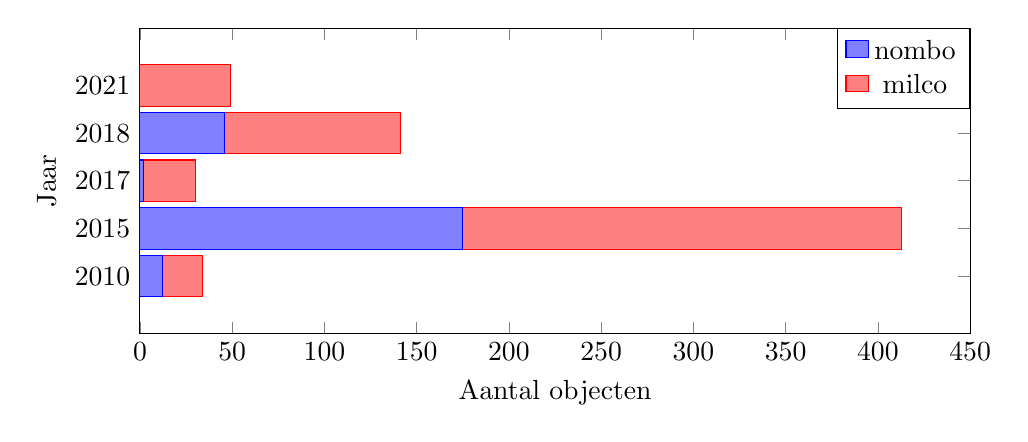
\begin{tikzpicture}
        \begin{axis}[
            xbar stacked,
            width=\textwidth,
            height=0.45\textwidth,
            symbolic y coords={2010, 2015, 2017, 2018, 2021},
            ytick=data,
            xmin=0,
            xmax=450,
            bar width=15pt,
            enlarge y limits=0.3,
            legend style={at={(1,1)}, anchor=north east, legend columns=1},
            xlabel={Aantal objecten},
            ylabel={Jaar}
            ]
            % First column data (Bottom part of stacked bars)
            \addplot+[xbar, color=blue, fill=blue!50] coordinates {(12,2010) (175,2015) (2,2017) (46,2018) (0,2021)};
            \addlegendentry{\glspl{nombo}}
            
            % Second column data (Top part of stacked bars)
            \addplot+[xbar, color=red, fill=red!50] coordinates {(22,2010) (238,2015) (28,2017) (95,2018) (49,2021)};
            \addlegendentry{\glspl{milco}}
            
        \end{axis}
    \end{tikzpicture}
    \caption[Aantal objecten per jaar in SSS for Mine Detection.]{\label{fig:SSSFMD_objects_per_year}Grafiek van het aantal waargenomen objecten per jaar in de \emph{\gls{sss} for Mine Data}-dataset. \autocite{Pessanha_Santos_2024}}
\end{figure}

Ook deze dataset wordt verspreid in een figshare-repository onder de CC BY 4.0 licentie. Opnieuw wordt een ZIP-archief van ongeveer 584 MB aangeboden. Dit ZIP-archief bevat opnieuw andere ZIP's. Deze hebben de naam van één van de jaren waarvan er data beschikbaar is en bevatten dit dan ook. Daarnaast is er nog een ZIP-bestand met de gewichten van een getraind \gls{YOLO}v4-model en de code hiervoor. Dit is echter niet nuttig voor dit onderzoek en zal dus niet gebruikt worden. \\

In de mappen verdeeld per jaar zitten zowel de beelden als de annotaties (niet gescheiden). De beelden zijn JPG-bestanden. Het lijkt erop dat er twee verschillende resoluties gebruikt zijn voor de afbeeldingen, namelijk \texttt{416 x 416} en \texttt{1024 x 1024}. De afbeeldingen volgen een vast benamingsschema: elke afbeelding bevat een oplopend nummer beginnend van \texttt{0001}, daarna een underscore en dan het jaar waarin de afbeelding is gemaakt. Alles samen is dat dus bijvoorbeeld: \texttt{0001\_2015.jpg}. De bestanden met annotatie staan in dezelfde map en hebben dezelfde naam als hun overeenkomstige afbeeldingen. Het enige verschil is dat zij een \texttt{.txt}-extensie hebben. Dit tekstbestand bevat de annotatie in \gls{yolo}-formaat. \autocite{Pessanha_Santos_2024_SSSFMD}

\begin{listing}[H]
    \begin{minted}{text}
        0 0.10009765625 0.2265625 0.0537109375 0.029296875
        1 0.43017578125 0.4443359375 0.0380859375 0.0546875
        0 0.587890625 0.7080078125 0.021484375 0.01953125
        0 0.84228515625 0.859375 0.0302734375 0.01953125
        1 0.17138671875 0.87890625 0.0244140625 0.017578125
        1 0.91455078125 0.958984375 0.0478515625 0.02734375
    \end{minted}
    \caption[YOLO-annotatie]{Voorbeeld van een TXT-bestand met annotatie voor objectdetectie in het YOLO-formaat (annotatie van \texttt{SSS for Mine Detection/2015/0001\_2015}). \autocite{Pessanha_Santos_2024_SSSFMD}}
\end{listing}

Eigenlijk is dit niks meer dan een CSV-bestand waarbij de separator een spatie is. In getabelleerde vorm is de data iets overzichtelijker.

\begin{table}[H]
    \centering
    \begin{tabular}{lllll}
        \toprule
        \textbf{Klasse} & \textbf{$x$-coördinaat} & \textbf{$y$-coördinaat} & \textbf{Hoogte} & \textbf{Breedte} \\
        \midrule
        0 & 0.10009765625 & 0.2265625    & 0.0537109375 & 0.029296875 \\
        1 & 0.43017578125 & 0.4443359375 & 0.0380859375 & 0.0546875   \\
        0 & 0.587890625   & 0.7080078125 & 0.021484375  & 0.01953125  \\
        0 & 0.84228515625 & 0.859375     & 0.0302734375 & 0.01953125  \\
        1 & 0.17138671875 & 0.87890625   & 0.0244140625 & 0.017578125 \\
        1 & 0.91455078125 & 0.958984375  & 0.0478515625 & 0.02734375  \\
        \bottomrule
    \end{tabular}
    \caption[YOLO-annotatie in getabelleerde vorm]{\label{tab:yolo_annot_table} Tabel met annotatie voor objectdetectie in het YOLO-formaat (annotatie van \texttt{SSS for Mine Detection/2015/0001\_2015}). \autocite{Pessanha_Santos_2024_SSSFMD}}
\end{table}

Merk op dat de klasse \texttt{0} of \texttt{1} is. Uit de paper van \textcite{Pessanha_Santos_2024} blijkt dat \texttt{0} een \gls{milco} is en \texttt{1} een \gls{nombo}. De volgende vier kolommen stellen een \gls{bounding_box} voor. Er bestaan verschillende formaten om zo'n \gls{bounding_box} voor te stellen. Dit formaat gebruikt één coördinaat ($(x, y)$) die het midden van de \gls{bounding_box} voorstelt, de hoogte en de breedte. \\

Men zou verwachten dat deze waarden gegeven zijn in pixels. Dat brengt echter een probleem met zich mee wanneer de afbeelding geschaald wordt. Dan moeten de pixelwaarden telkens herberekent worden om zo de \gls{bounding_box} op de juiste plaats op de afbeelding te laten vallen. Om dit op te lossen worden deze waarden -- zoals hier -- meestal als verhoudingen uitgedrukt. Zo is de breedte bijvoorbeeld de breedte in pixels gedeeld door de breedte van de afbeelding.

\begin{figure}[H]
    \centering
    \begin{tikzpicture}
        
        % Draw the outer rectangle (image)
        \draw[thick] (0,0) rectangle (7,7);
        % Label the dimensions of the outer rectangle
        \draw[<->] (-0.5,0) -- (-0.5,7) node[midway, left] {$h_{image}$};
        \draw[<->] (0,-0.5) -- (7,-0.5) node[midway, below] {$w_{image}$};
        
        % Draw the bounding box inside the image
        \draw[thick, dashed] (2,2) rectangle (5,5);
        % Label the dimensions of the bounding box
        \draw[<->] (1.5,2) -- (1.5,5) node[midway, left] {$h_{bb}$};
        \draw[<->] (2,1.5) -- (5,1.5) node[midway, below] {$w_{bb}$};
        
        % Add a dot in the center of the bounding box
        \filldraw [black] (3.5,3.5) circle (2pt);
        % Label the coordinates of the dot
        \node at (3.5,3) {$(x_{bb}, y_{bb})$};
        
    \end{tikzpicture}
    \caption[Structuur van een bounding box.]{\label{fig:bounding_box}Structuur van een \gls{bounding_box} (gebaseerd op een figuur van \textcite{Pessanha_Santos_2024})}.
\end{figure}

Als de afbeelding geschaald wordt, schaalt de \gls{bounding_box} mee en kan men aan de hand van een relatief eenvoudige formule terug de pixelwaarde berekenen zonder complexe transformaties op de \gls{bounding_box} te moeten gaan toepassen. De formule om de absolute pixelwaarden om te zetten naar relatieve verhoudingen is de volgende:

$$
(x,y,w,h) = \left(\frac{x_{bb}}{w_{image}},\frac{y_{bb}}{h_{image}},\frac{w_{bb}}{w_{image}},\frac{h_{bb}}{h_{image}}\right)
$$ 

\clearpage

Naast het verzamelen van de dataset trainden de onderzoekers ook een objectdetectiemodel -- namelijk \gls{yolo}v4 -- op deze data om de kwaliteit ervan te testen. De configuratie voor het trainingsproces werd speciaal aangepast om de performance van dit model te verhogen. De \gls{batch_size} werd ingesteld op 64 en werden gedurende de training opgesplitst in 16 \glspl{mini_batch} van elk 4 afbeeldingen, dit om het geheugengebruik tijdens het trainingsproces te optimaliseren. \\

Het maximum aantal \glspl{batch} werd ingesteld op 6000. Ook werd de \gls{learning_rate} van het model op kritieke punten aangepast, namelijk na het verwerken van 4800 en 5400 \glspl{batch}, dit om de convergentie te verhogen. Ook pasten de onderzoekers transfer learning toe door de gewichten van het model te initialiseren met gewichten van de \gls{coco}-dataset. Na het model te trainen op de volledige dataset van 1170 afbeeldingen, behaalde deze een \gls{iou} van 60\% en een \gls{map} van 75\%. Ook werd een \gls{precision} van 82\% en een \gls{recall} van 64\% behaald. \autocite{Pessanha_Santos_2024}

\subsubsection{UXO}

Ten slotte is er de \acrshort{uxo}-dataset. \acrshort{uxo} is de afkorting voor \acrlong{uxo}, de Engelse benaming voor \glspl{blindganger}. Dit is meteen ook de inhoud van deze dataset. Ze bevat namelijk 74 437 afbeeldingen van \glspl{blindganger} en is daarmee de grootste dataset die in dit onderzoek voorkomt. Het doel van deze dataset is om een validatieset te zijn en ze is samengesteld om onderzoek naar ontmijning in plassen, meren, zeeën en oceanen vooruit te helpen. Zoals al eerder vermeld is dit onderwerp zeer gevoelig en wordt er meestal (lees: bijna altijd) voor gekozen om deze datasets zo confidentieel mogelijk te houden. Daarom bevat deze dataset ook geen \emph{real-world}-afbeeldingen. In plaats daarvan zijn beelden in een gecontroleerde, experimentele omgeving gemaakt. \autocite{Dahn_2024_UXO}

\begin{figure}[H]
    \centering
    \includegraphics[width=\textwidth]{teaser_uxo.png}
    \caption[Voorbeeld van sonarbeelden \& afbeeldingen in de UXO-dataset]{\label{fig:uxo_teaser}. Voorbeeld van sonarbeelden en overeenkomstige afbeeldingen van verschillende type \glspl{blindganger} in de UXO-dataset. \autocite{Dahn_2024_UXO}}
\end{figure}

Om deze dataset samen te stellen, hebben de onderzoekers een volledig gecontroleerde testopstelling gemaakt bij het \gls{dfki}, het Duits onderzoekscentrum voor artificiële intelligentie in Bremen. De dataset is gemaakt met een ARIS Explorer 3000 sonarmodule (voor de sonarbeelden) en een GoPro Hero 8 (voor de bijhorende 5,3K UHD afbeeldingen). Deze twee modules werden op een \gls{PTU} (de ARIS Rotator AR3) gemonteerd die vastzat aan een op maat gemaakte \gls{portaalkraan}. Deze kraan kon vrij in de $xyz$-assen bewegen en kon verschillende voorgeprogrammeerde banen heel precies volgen. Om de omgeving van de zee zo goed mogelijk te kunnen nabootsen, bouwden de onderzoekers een bassin gevuld met 20 000 liter zoetwater. Hierin plaatsten ze verschillende \emph{targets}, de \glspl{blindganger}. Deze waren aangeleverd door EGGERS Kampfmittelbergung GmbH, een bedrijf dat zich bezighoudt met het ontmijnen van verschillende sites. Om de veiligheid te garanderen, werden de \glspl{blindganger} voordien onschadelijk gemaakt. Er werden verschillende \glspl{blindganger} gebruikt om zo variëteit in de dataset te garanderen: een normale bom van ongeveer 51 kg, een vervormde fosforbom en een mortier. \autocite{Dahn_2024}

\begin{figure}[H]
    \centering
    \includegraphics[width=0.5\textwidth]{uxo_setup.jpg}
    \caption[Setup waarmee de UXO-dataset gemaakt is]{\label{fig:uxo_setup}. Afbeelding van de setup die gebruikt werd om data te verzamelen voor de UXO-dataset. \autocite{Dahn_2024_UXO}}
\end{figure}

De dataset is alles samen zo'n 94,7 GB groot. Ze is de meest uitgebreide die in dit onderzoek voorkomt, niet alleen qua grootte, maar ook qua inhoud. De dataset is onderverdeeld in verschillende mappen. De map \texttt{3d\_models} bevat 3D-modellen van de \glspl{blindganger}. De map \texttt{calibration} bevat dan weer de transformaties tussen de kraan en de sensors en de kalibraties van de GoPro. Het merendeel van de dataset zit in de map \texttt{recordings}. Deze bevat mappen per type \gls{blindganger}. In deze mappen zitten dan telkens weer mappen met de datum en tijd van elk experiment. Deze mappen bevatten verschillende mappen en bestanden die de \emph{core} van de data vormen. \autocite{Dahn_2024_UXO}

\clearpage

\begin{itemize}
    \item \textbf{\texttt{aris\_raw}:} map die de \emph{raw} sonarbeelden bevat in PGM formaat. Dit is een eenvoudig rasterafbeeldingsformaat (zoals BMP, cf. figuur \ref{fig:bitmap_example_image}) dat grijswaardenafbeeldingen opslaat. PGM-bestanden kunnen in een ASCII (tekst) of binaire (snellere) variant worden opgeslagen. Elke pixel heeft een intensiteitswaarde tussen 0 (zwart) en een maximumwaarde (meestal 255, wit), waardoor verschillende grijstinten mogelijk zijn. De afbeelding bevat ook een header met het formaat, afmetingen en maximale intensiteit, gevolgd door de pixelgegevens. PGM wordt vaak gebruikt in beeldverwerking en wetenschappelijke toepassingen vanwege de eenvoud en brede compatibiliteit. \autocite{Poskanzer_2016}
    \item \textbf{\texttt{aris\_polar}:} map die de poolgetransformeerde sonarbeelden bevat in PNG formaat.
    \item \textbf{\texttt{gopro}:} map die de beelden in JPG formaat bevat die gemaakt zijn door de GoPro.
    \item \textbf{\texttt{labels}:} map die annotatie van \glspl{bounding_box} bevat in JSON formaat.
    \item \textbf{\texttt{aris\_file\_meta.yaml}:} YAML-bestand met de metadata van de sonar 
    \item \textbf{\texttt{aris\_frame\_meta.csv}:} CSV-bestand met metadata voor elk sonarframe, inclusief \gls{ptu}-informatie.
    \item \textbf{\texttt{gantry.csv}:} CSV-bestand met posities van de \gls{portaalkraan} bij elk sonarframe.
    \item \textbf{\texttt{notes.txt}:} TXT-bestand met korte beschrijving over experiment.
\end{itemize}

\begin{figure}[H]
    \centering
    \includegraphics[width=0.5\textwidth]{uxo_preview.jpg}
    \caption[UXO-setup in actie]{\label{fig:uxo_preview}. Preview van de setup waarmee de UXO-dataset is gemaakt in actie. \autocite{Dahn_2024_UXO}}
\end{figure}

\clearpage

\subsubsection{Conclusie}

Alle drie de datasets die hierboven besproken werden, maken het mogelijk om een objectdetectiemodel mee te trainen. Ze bieden namelijk allemaal annotaties van \glspl{bounding_box} op de bijhorende afbeeldingen aan. Daarnaast zijn deze datasets makkelijk te verwerken, aangezien alle beelden in conventionele afbeeldingsformaten zijn opgeslagen (zoals PNG, JPG, BMP, PGM, \dots). Toch is er -- specifiek voor dit onderzoek -- één dataset die geschikter is dan de anderen. De UATD-dataset is -- misschien ietwat subjectief -- uitgekozen om te gebruiken in de rest van dit onderzoek. Dit komt omdat ze bepaalde aspecten aanbiedt die de andere datasets niet hebben. \\

\gls{sss} for Mine Detection lijkt op het eerste zicht de perfecte dataset voor dit onderzoek. Het probleem is echter dat ze relatief klein is: ze bevat ``slechts'' 1170 afbeeldingen. Op het eerste zicht lijkt dit voldoende. Echter moet deze dataset nog opgesplitst worden in -- ten minste -- een trainingsset en een testset.\footnote{In een optimale situatie zou de data opgesplitst worden in drie sets: een trainingsset, een testset en een validatieset. Dit komt omdat de validatiedataset -- hoewel ze niet gebruikt wordt om het model te trainen -- gebruikt wordt om de paramaters van het model te tunen. Dit kan leiden tot \gls{overfitting}. Het is beter om als testset data te gebruiken dat het model nog niet gezien heeft. \autocite{Goodfellow_2016}} Ook komen er slechts 668 objecten voor in de dataset. Tot overmaat van ramp zijn deze ook zeer slecht verdeeld. 

\begin{table}[H]
    \centering
    \begin{tabular}{ll}
        \toprule
        \textbf{\# objecten / beeld} & \textbf{\# beelden} \\
        \midrule
        13 & 1 \\
        9  & 2 \\
        8  & 4 \\
        7  & 8 \\
        6  & 8 \\
        5  & 13 \\
        4  & 9 \\
        3  & 41 \\
        2  & 59 \\
        1  & 159 \\
        0  & 866 \\
        \bottomrule
    \end{tabular}
    \caption[Aantal objecten per afbeelding in SSS for Mine Data]{\label{tab:objects_per_image_sss} Tabel met verdeling van objecten per afbeelding in de \gls{sss} for Mine Detection-dataset.}
\end{table}

\clearpage

Er is één afbeelding met wel 13 objecten en 866 zonder ook maar één object. Door deze slechte verdeling en de beperkte hoeveelheid data in de dataset is ze dus weinig bruikbaar voor dit onderzoek. \\

Dit is een probleem waar de UXO-dataset absoluut niet mee kampt. Deze heeft dan echter weer andere problemen. De dataset is namelijk volledig samengesteld in een gecontroleerde testopstelling. Ze bevat dus geen \emph{real-world}-data. Dit betekent echter ook dat bepaalde artefacten en afwijkingen typisch aan meren en zeeën niet in deze dataset voorkomen. De beelden zijn zodanig zuiver dat het hoogstwaarschijnlijk mogelijk zou zijn om de \glspl{blindganger} te herkennen door te zoeken naar de groep helderste pixels of met een edge-detection algoritme. \autocite{Torre_1986} \\

Ook de grootte van de dataset is misschien iets te mooi om waar te zijn. De beelden in de dataset zijn namelijk geen onafhankelijke afbeeldingen, maar frames van een continue opname. Dit zorgt ervoor dat er (nagenoeg) geen verschil is tussen afbeelding $n$ en afbeelding $n+1$. Als alle afbeeldingen na elkaar worden afgespeeld, ziet men een opname van een transformatie (rotatie, verschuiving, \dots) van één van de \glspl{blindganger}. Ten slotte staat er telkens maar één object op een afbeelding, wat multiple objectdetectie (meerdere objecten op één afbeelding herkennen) onmogelijk maakt.